
%%%%%%%%%%%%%%%%%%%%%%% file typeinst.tex %%%%%%%%%%%%%%%%%%%%%%%%%
%
% This is the LaTeX source for the instructions to authors using
% the LaTeX document class 'llncs.cls' for contributions to
% the Lecture Notes in Computer Sciences series.
% http://www.springer.com/lncs       Springer Heidelberg 2006/05/04
%
% It may be used as a template for your own input - copy it
% to a new file with a new name and use it as the basis
% for your article.
%
% NB: the document class 'llncs' has its own and detailed documentation, see
% ftp://ftp.springer.de/data/pubftp/pub/tex/latex/llncs/latex2e/llncsdoc.pdf
%
%%%%%%%%%%%%%%%%%%%%%%%%%%%%%%%%%%%%%%%%%%%%%%%%%%%%%%%%%%%%%%%%%%%


\documentclass[runningheads,a4paper]{llncs}

\usepackage{amsmath,amssymb}
\let\doendproof\endproof
\renewcommand\endproof{~\hfill\qed\doendproof}

\setcounter{tocdepth}{3}
\usepackage{graphicx}
%\usepackage{indentfirst}
\usepackage[linesnumbered,boxed,ruled]{algorithm2e}


\usepackage{url}
\urldef{\mailsa}\path|{alfred.hofmann, ursula.barth, ingrid.haas, frank.holzwarth,|
\urldef{\mailsb}\path|anna.kramer, leonie.kunz, christine.reiss, nicole.sator,|
\urldef{\mailsc}\path|erika.siebert-cole, peter.strasser, lncs}@springer.com|    
\newcommand{\keywords}[1]{\par\addvspace\baselineskip
\noindent\keywordname\enspace\ignorespaces#1}

\begin{document}

\mainmatter  % start of an individual contribution

% first the title is needed
\title{Cloud-oriented SAT Solver based on obfuscating CNF}

% a short form should be given in case it is too long for the running head
%\titlerunning{Lecture Notes in Computer Science: Authors' Instructions}

% the name(s) of the author(s) follow(s) next
%
% NB: Chinese authors should write their first names(s) in front of
% their surnames. This ensures that the names appear correctly in
% the running heads and the author index.
%
\author{Ying Qin%
% \thanks{Please note that the LNCS Editorial assumes that all authors have used
% the western naming convention, with given names preceding surnames. This determines
% the structure of the names in the running heads and the author index.}%
\and ShengYu Shen\and Yan Jia}
%
% \authorrunning{Lecture Notes in Computer Science: Authors' Instructions}
% (feature abused for this document to repeat the title also on left hand pages)

% the affiliations are given next; don't give your e-mail address
% unless you accept that it will be published
\institute{National University of Defense Technology, School of Computer Science,\\
ChangSha, China\\
%\mailsa\\
%\mailsb\\
%\mailsc\\
\url{http://www.nudt.edu.cn}}

%
% NB: a more complex sample for affiliations and the mapping to the
% corresponding authors can be found in the file "llncs.dem"
% (search for the string "\mainmatter" where a contribution starts).
% "llncs.dem" accompanies the document class "llncs.cls".
%

\toctitle{Lecture Notes in Computer Science}
\tocauthor{Authors' Instructions}
\maketitle

\begin{abstract}

Propositional satisfiability (SAT) has been widely used in hardware and software verification. 
Outsourcing complex SAT problem to Cloud can leverage the huge computation capability and flexibility of Cloud.
But some confidential information encoded in CNF formula, 
such as circuit structure, 
may be leaked to unauthorized third party.

In this paper, we propose a novel Cloud-oriented SAT solving algorithm to preserve privacy.
$\mathbf{First}$, an obfuscated CNF formula is generated by embedding a Husk formula into the original formula with proper rules.
$\mathbf{Second}$, the obfuscated formula is solved by a state-of-the-art SAT solver deployed in Cloud.
$\mathbf{Third}$, a simple mapping algorithm is used to map the solution 
of the obfuscated formula back to that of the original CNF formula. 

Theoretical analysis and experimental result show that our algorithms can significantly improve security of the SAT solver 
with linear complexity while keeping its solution space unchanged.


\keywords{SAT solver; CNF formula; Privacy; Obfuscating; Cloud computing}
\end{abstract}

\section{Introduction}
Propositional satisfiability \cite{t1} (SAT) has been widely used in hardware and software verification \cite{t2}\cite{t3}. 
With the rapid increase of the hardware and software system size,
the size of SAT problem generated from verification also increases rapidly. 

On the other hand, 
Cloud computing can provide elastic computing resource,
which make outsourcing hard SAT problem 
to public Cloud \cite{t35}\cite{t37} very attractive.
However,
% when outsourcing SAT solving,
% computing data shall be send into remote server which is shared among different client. 
unauthorized access to outsourced data prevent it from widely deployed. 

In formal verification, 
circuit, code and properties will first be converted into CNF (Conjunctive Normal Form) formula 
by Tsentin coding\cite{t4} before SAT solving. 
After that, 
circuit structure and other confidential information are still existed in CNF formula.
To prevent unauthorized user from accessing these confidential information, 
it is necessary to obfuscate CNF formula before outsourcing.

This paper presents a novel Cloud SAT solver based on Obfuscating CNF.
\textbf{First}, 
the original CNF formula $S_1$ is obfuscated into another formula $S$
by embedding another CNF formula $S_2$ with unique solution.
And the embedding rules guarantee that $S$'s graph structure are significantly different from that of $S_1$.
\textbf{Second},
$S$ is sent to a SAT solver in Cloud, 
which returns a solution $R_O$.
\textbf{Third}, 
the solution $R$ of $S_1$ is obtained from the solution of $R_O$ by projection.
its correctness can be guaranteed by the embedding rules in the first step.

The major contributions of this paper are:
\textbf{First}, by obfuscating, 
confidential information in the original CNF formula,
such as circuit structure, 
will be destroyed in the obfuscated CNF formula; 
\textbf{Second}, 
the obfuscated CNF formula can be solved by state-of-the-art SAT solver. 
\textbf{Third}, 
the theoretical analysis and experiments shows that obfuscating and solution recovery algorithms linear complexity, 
reducing the impact on the overall performance of SAT solving.

The remainder of this paper is organized as follows.
Background material is presented in Section \ref{prep}.
Section \ref{problem} gives the description of the problem, 
while the implementation of Cloud SAT solver based on obfuscating is presented in Section \ref{algo}.
Section \ref{correct} analyzes correctness, effectiveness and complexity; 
Section \ref{related} describes the related work; 
Section \ref{exp} gives the experimental results,
while Section \ref{conclude} concludes this paper.


\section{Preliminaries}\label{prep}
\subsection{SAT solving}

The Boolean value set is denoted as $B=\{T,F\}$. 
For a Boolean formula $S$ over a variable set $V$, 
the propositional satisfiability problem (abbreviated as SAT) is 
to find a satisfying assignment $A : V\to B$, 
so that $S$ evaluates to $T$. 
If such a satisfying assignment exists, 
then $S$ is satisfiable; 
otherwise,
it is unsatisfiable.
A clause subset of an unsatisfiable formula is an unsatisfied core.
A computer program that decides the existence of a
satisfying assignment is SAT solver\cite{t10}.

Normally, 
a SAT solver requires the formula to be  conjunctive normal form (CNF), 
in which a formula is a conjunction of its clause set, 
and a clause is a disjunction of its literal set, 
while a literal is a variable or its negation.


$\Phi$ in Equation (\ref{eqn_phi}) is a CNF formula 
with four variables $x_1$, $x_2$, $x_3$, $x_4$, 
and four clauses $x_1\vee \neg x_2$, $x_2\vee x_3$, $x_2\vee \neg x_4$, $ \neg x_1\vee \neg x_3\vee x_4$.
% In clause $x_1\vee \neg x_2$, there are two literals $x_1$ and $ \neg x_2$.
Literal $x_1$ is positive literal of variable $x_1$ in clause $x_1\vee \neg x_2$,
while $ \neg x_2$ is a negative literal.

\begin{equation}\label{eqn_phi}
\centering \Phi=(x_1\vee \neg x_2)\wedge(x_2\vee x_3)\wedge(x_2\vee \neg x_4)\wedge( \neg x_1\vee \neg x_3\vee x_4)
\end{equation}

The number of literals in clause $C$ is denoted as $|C|$.
The number of clauses in a CNF formula $F$ is denoted as $|F|$.
For example $| x_1\vee  \neg x_2 |\equiv 2$,
while $|\phi|\equiv 4$

\subsection{Tseitin encoding}

In hardware verification, 
circuits and properties are converted into CNF formula by Tseitin encoding\cite{t4},
and then CNF formula is solved by SAT solver.
Circuits can all be expressed by a combination of gate AND2 and INV, 
so we only lists Tseitin encoding of gate AND2 and INV here. 

For gate INV $z=\neg x$, 
its Tseitin encoding is  $(x\vee z)\wedge( \neg x\vee \neg z)$.
For gate AND2 $z=x_1\wedge x_2$, 
its CNF formula is $( \neg x_1\vee \neg x_2\vee z)\wedge(x_1\vee \neg z) \wedge(x_2\vee \neg z)$.
% For other type gate, its according CNF formula can be generated through Tseitin encoding.
For a complex circuit $C$ expressed by a combination of AND2 and INV, 
its Tseitin encoding $Tseitin(C)$ is a conjunctive of all these gates' Tseitin encoding.

% The circuit in Figure \ref{fig_tseitin}a) consists of a gate AND and a gate OR.
% Tseitin encoding of this circuit is shown in Figure \ref{fig_tseitin}b) and Figure \ref{fig_tseitin}c).
% Formally, 
% for any circuit $C$, 
% its Tseitin encoding is denoted as $Tseitin(C)$.
% 
% \begin{figure}
% \centering
% \includegraphics[width=7.2cm]{a1}
% \caption{Tseitin encoding of circuit}
% \label{fig_tseitin}
% \end{figure}

For a circuit $C$ with an INV $d=\neg a$ and an AND2 $e=d\wedge c$,
its Tseitin encoding is shown in Equation (\ref{eqn_andinv}).
\begin{equation}\label{eqn_andinv}
Tseitin(C)=\left\{
\begin{array}{cc}
& (a\vee d) \\
\wedge & (\neg a\vee \neg d)
\end{array}
\right\}\wedge\left\{
\begin{array}{cc}
& (\neg e\vee c) \\
\wedge & (\neg e\vee d) \\
\wedge & (e\vee \neg c\vee\neg d)
\end{array}
\right\}
\end{equation}

% This paper focuses on obfuscating of CNF formula generated from circuit in formal verification, the obfuscating algorithm is also suitable for CNF formula generated from software code.

% \section{Problem Definition}
\section{Threat Model of Cloud-based SAT solving}\label{problem}

Solving SAT in Cloud includes three steps:
\textbf{first} generating and uploading CNF formula to Cloud, 
\textbf{then} solving CNF in Cloud,
\textbf{finally} downloading solution.
Thus,
unauthorized access\cite{t11} to CNF formula in Cloud may result in leakage of confidential information.

%, as illustrated in Fig. 2.
%\begin{figure}
%\centering
%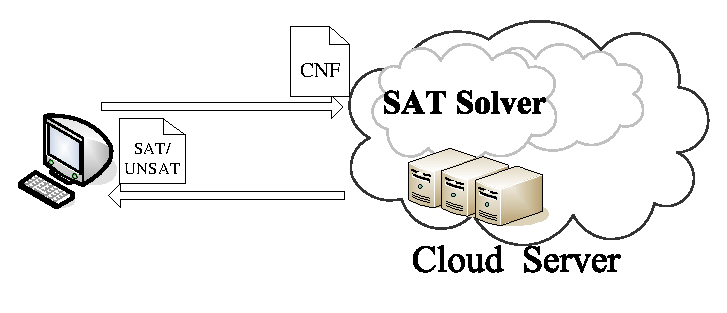
\includegraphics[width=7.2cm]{a2}
%\caption{SAT solving in Cloud }
%% %\label{fig:example}
%\end{figure}
% As illustrated in Fig. 2.
% \begin{figure}
% \centering
% 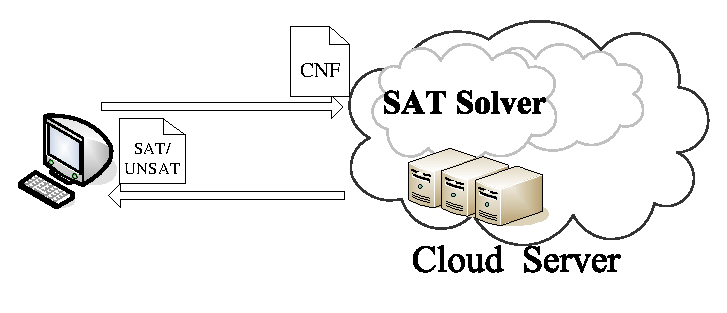
\includegraphics[width=6.2cm]{a2}
% \caption{SAT solving in Cloud }
% % %\label{fig:example}
% \end{figure}

% \begin{enumerate}
% \end{enumerate}


% In Cloud computing paradigm, CNF formula will be uploaded and handled in public Cloud; 
% Cloud are multi-tenant, unauthorized access\cite{t11} to CNF formula may result in leakage of sensitive information.


On the other hand,
verifying the result of SAT is simple.
If CNF formula is satisfiable, 
the solution can be substituted into CNF to check if it is satisfiable;
If CNF formula is unsatisfiable, 
an unsatisfiable core returned by the SAT solver can be verified by resolution.
In both case,
verifying the result are linear complexity.

Thus, in this paper we assume that Cloud servers are honest but curious.
That is,
the CNF will be solved correctly, 
but also may be analyzed to recover confidential information.
% The circuit structure is not lost during Tseitin encoding. 
Algorithms \cite{t6,t7,t8,t9} have been proposed to recover circuit from CNF.
Before discussing them,
some concepts should be introduced first.  

\begin{definition}[CNF signature]
% A CNF signature of a gate is a CNF formula representing the characteristic function of the gate.
CNF signature of gate $g$ is its Tseitin encoding $Tseitin(g)$.
Each clause in CNF signature is called characteristic clause.
A characteristic clause containing all variables in CNF-signature is a \textbf{key clause}.
Variables correspond to output of a gate is called \textbf{output variable}.
\end{definition}


For AND2 in Equation (\ref{eqn_andinv}),
$\neg e\vee c$ is a characteristic clause. 
Clause $e\vee \neg c\vee\neg d$ is a key clause. 
$e$ is an output variable.
% For example,
% three input AND gate (AND3) is converted into its CNF signature $C$ shown in Equation (\ref{eqn_and3}).
% $c_1 \sim c_4$ is a characteristic clause. 
% Clause $c_1$ that contains all the variables is a key clause. 
% $a$ is an output variable.

% \begin{equation}\label{eqn_and3}
% a=b\wedge c\wedge d \longrightarrow C=\left\{
% \begin{array}{rl}
% c_1 : & a\vee \neg b\vee \neg c\vee \neg d\\
% c_2 : & \neg a \vee b\\
% c_3 : & \neg a \vee c\\
% c_4 : & \neg a \vee d
% \end{array}
% \right\}
% \end{equation}

% \begin{figure}
% \centering
% \includegraphics[width=7.2cm]{a3}
% \caption{CNF signature of gate AND3 }
% \label{fig_and3}
% \end{figure}

With such encoding rules, 
gates with the same CNF signature will be encoded into the same set of clauses. 
Potential attackers can exploit structural knowledge to recover the circuit structure. 
Some such algorithms\cite{t6,t7,t8,t9} are based on concept of directed hyper-graph and bipartite graph described below.

\begin{definition}[Hypergraph of CNF and Directed Hypergraph of CNF]
A Hypergraph $G=(V,E)$ of a CNF formula $\Sigma$ is
\begin{enumerate}
 \item each vertex of $V$ corresponds to a clause of $\Sigma$;
 \item each edge $(c_1,c_2)\in E$ corresponds to two clauses $c_1$ and $c_2$ containing the same variable or its negation;
 \item each edge is labeled by the variable;
\end{enumerate}
A Directed Hypergraph is a Hypergraph with each endpoint of edge labeled 
by $\uparrow$ when clause contains non-negative variable,
or $\dag$ when clause contains negative variable.
\end{definition}


 \begin{definition}[Bipartite graph of CNF]
 A Bipartite graph $G=(V,E)$ of a CNF formula $\Sigma$ is
\begin{enumerate}
 \item each vertex of $V$ corresponds to clause and variable of $\Sigma$;
 \item each edge $(c,v)\in E$ corresponds to a clauses $c$ that contains variable $v$;
 \item each edge is labeled by  $\uparrow$  when clause contains non-negative variable, or
$\dag$ when clause contains negative variable.
\end{enumerate}
\end{definition}


% Fig.4a) gives the corresponding hypergraph of gate AND3 in Fig.3. 
% Fig.4b) gives the corresponding Directed Hyper-Graph of gate AND3 in Fig.3. while $\uparrow$ represents positive, - represents negative variable.
% Fig.4c) gives the corresponding Bipartite Graph of gate AND3 in Fig.3.
% \begin{figure}
% \centering
% 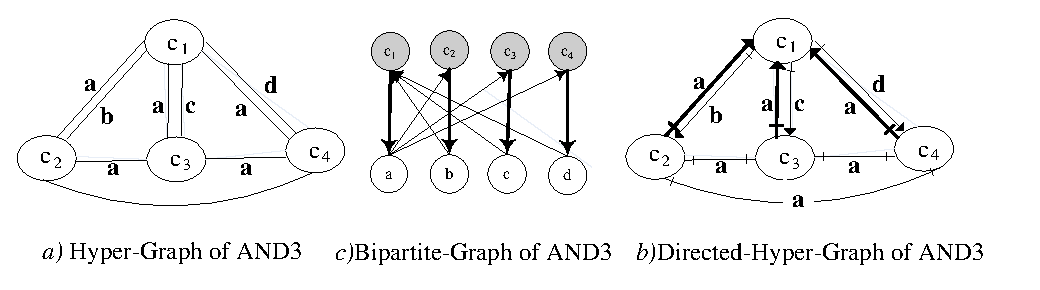
\includegraphics[width=7.2cm]{a4}
% \caption{Graph representation of gate AND3}
% %%\label{fig:example}
% \end{figure}
% 
With these definitions, 
Roy et al. \cite{t8} 
% articulats that an arbitrary combinational circuit can be encoded as a CNF-SAT instance 
% so that its circuit structure is preserved and can readily be extracted. 
% they 
% describes an algorithm to recover circuit structure from CNF:
% and empirically show its success and scalability on very large benchmarks. 
% The basic steps in their Generic Circuit Detection algorithm are as follows 
% 
first converts the CNF to an Hypergraph $G$,
and then matches the CNF signatures of all types of gates in $G$ to recover gates by subgraph isomorphism,
finally creates a maximal independent set (MIS) instance to represent the recovered circuit.

Fu et al.\cite{t9} presents another algorithm that 
% The CNF2CKT algorithm effciently extracts a maximum circuit structure from any given CNF instance. 
%Some important features of CNF2CKT are:
first detects all possible gates with pattern matching,
and then constructs a maximum acyclic combinational circuit by selecting a maximum subset of matched gate.
%  , i.e. a cover, 
%  from all the candidate matchings. 
%  Maximum here is with respect to the number of logic gates in the extracted circuit, i.e. the size of the cover, 
%  since one matching corresponds to one logic gate in the extracted circuit. 
%  The cover is maximum in the sense that no other circuit structure containing more logic gates can be extracted from the CNF description.

% All state-of-the-art algorithms\cite{t6,t7,t8,t9} recover circuit structure 
% by exploiting the graph structure characteristics of CNF formula,
% such as subgraph isomorphism and pattern matching.
In Cloud computing paradigm,
attacker may use these algorithms to recover the circuit structure from CNF formula.
Therefore, 
it is essential to prevent information leakage before outsourcing CNF formula to Cloud.

\section{Cloud-based SAT solver preserving privacy}\label{algo}

In this paper, we present a Cloud-based SAT solver based on obfuscating, 
which prevent information leakage by hiding the structure in CNF.
The obfuscating algorithm is based on the following three facts:
\begin{enumerate}
 \item First, 
%  since CNF signature is key in circuit recovering, 
 changing CNF signature of gates in CNF formula will make circuit recovering 
 based on pattern matching or subgraph isomorphism impossible.
 \item Second, 
 current SAT solver with conflict analysis \cite{t10} is very efficient.
So we would like to use them directly,
instead of developing a new one like \cite{t11}.
 \item Third,
 the solution of obfuscated CNF formula should be easily mapped back to original formula.
\end{enumerate}

The proposed algorithm is based on the following definition.

%\noindent Definition 5: Husk formula is a CNF formula with a unique solution,in which assignment of variables is non-specific(Not all 0 or all 1).
\begin{definition}[Husk formula]
Husk formula is a CNF formula with a unique solution,
and assignment of variables is non-uniform,
that is,
not all 0 or all 1.
\end{definition}

The overall framework of the Cloud SAT solver is shown intuitively in Figure \ref{fig_cldSAT}.
In Step 1,
GENERATOR algorithm generates a husk formula with unique solution $R_H$;
In Step 2,
OBFUSCATOR algorithm obfuscates $S_1$ to obtain a new CNF formula $S$;
In Step 3,
$S$ is solved in Cloud;
In Step 4,
MAPPER algorithm maps solution of $S$ to that of $S_1$.

% and formally in Algorithm \ref{algo1}.
% Steps 1, 2 and 4 are done locally,
% while step 3 is in Cloud.

\begin{figure}
\centering
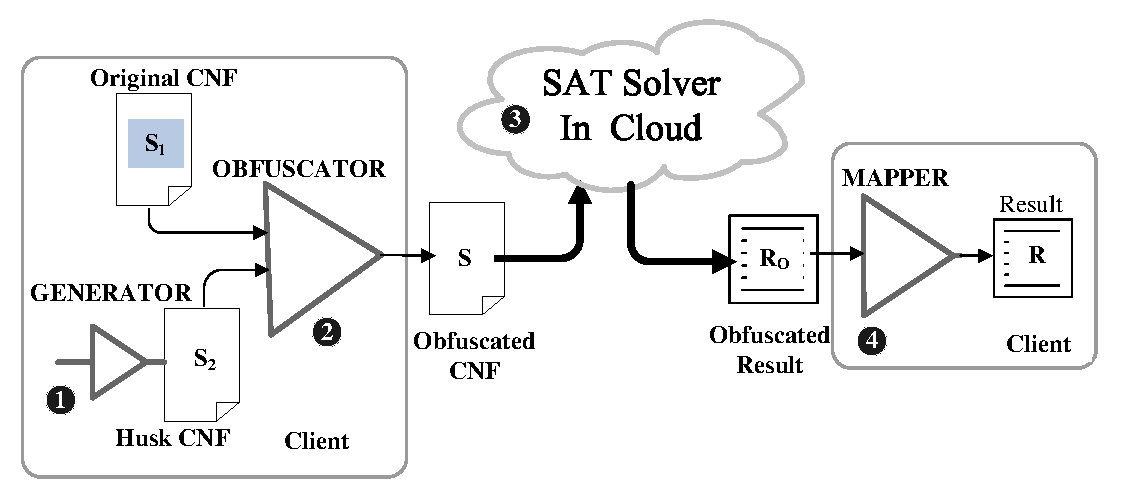
\includegraphics[width=7.2cm]{a5}
\caption{The Cloud SAT solver based on obfuscating CNF}
\label{fig_cldSAT}
\end{figure}


% \begin{algorithm}[t]
% \KwData{The original CNF formula $S_1$ }
% \KwResult{The solution of $S_1$}
% \Begin{
%  \;
%  \;
%  \;
%  \;
% }
% \caption{The general framework}
% \label{algo1}
% \end{algorithm}


The GENERATOR, OBFUSCATOR and MAPPER algorithm will be described in Subsection \ref{genhusk},\ref{obfuscating} 
and \ref{mappping} respectively.
% It need be emphasized that, $S_1$  and $S_2$ have disjoint set of variables.

\subsection{Generating Husk formula}\label{genhusk}
% From the point of view of cryptology, Husk formula is a secret key used to encrypt the CNF formula. 
% Our obfuscating algorithm requires Husk formula has a unique solution.
% In this paper, 
Husk formula is constructed based on prime factorization method:
\textbf{First},
given a prime $p$ represented by a binary vector $p = <p_1,p_2,\dots,p_n>$, 
we assigning its square $p^2$ to the output of a multiplier $M$, 
with constraint $p\ne 1$.
\textbf{Second},
We convert the multiplier $M$ into CNF formula $Tseitin(M)$.

To satisfy $Tseitin(M)$,
the two inputs of $M$ must all be $p = <p_1,p_2,\dots,p_n>$,
which makes the $p$ the unique solution of $Tseitin(M)$.

With these discussion,
GENERATOR algorithm to generate Husk formula is shown in Algorithm \ref{algo2_gen}.

\begin{algorithm}[b]
\SetAlgoLined
\KwData{NULL}
\KwResult{Husk CNF $S_2$ and Husk result $R_H$}
\Begin{
Generating a prime number $p$ \;
% $sq=p\times p$ \;
$\Phi= M(I_1 \neq 1, I_2\neq 1, O=p^2)$ \;
$S_2=Tseitin(\Phi)$ \;
$R_H=p\mid p$ \;
}
\caption{GENERATOR}
\label{algo2_gen}
\end{algorithm}


\subsection{Constructing obfuscated formula}\label{obfuscating}

The proposed OBUFSCATOR algorithm generates a new CNF formula $S$
by embedding Husk formula $S_2$ into the original formula $S_1$ with proper rules.
% (there is no intersection between variables set of $S_2$ and $S_1$). 
By adding new clauses and new literals, 
OBUFSCATOR algorithm changes the clause set and literal set in clauses of $S_1$,
to prevent its structure from being recovered.


\begin{algorithm}[t]
\KwData{The original CNF $S_1$,Husk CNF $S_2$,Husk result $R_H$}
\KwResult{The obfuscated CNF $S$, variable mapping $M$}
\Begin{
$mark(S_1)$\;\label{mark}
\ForEach{$c\in S_1$}{
lit =get literal $ \in R_H$\;
$c=c \cup \neg lit$\;\label{rule1}
\If{$c \in$  Key Clause Set KCS} {
$nc=generate\_new\_clause(c,lit)$\;\label{gennewclause}
$S_2=S_2 \cup nc$\;
}
}
\ForEach{$ c \in S_1 $} {
$averagelen=\frac{\sigma _{c'\in S_1}|c'|}{|S_1|}$ \;
\While{$|c| < averagelen$}{
$lit=$get literal $\in R_H$ \;
\While{$\neg lit \in c$} {
lit=get literal $ \in R_H $ \;
}
$c=c \cup \neg lit$\;\label{rule2}
}
$M$ =remap all variable in $S_1\cup S_2$ \;
$S$ =reorder all clause in $S_1\cup S_2$ \;
}
}
\caption{OBFUSCATOR}
\label{algo_obs}
\end{algorithm}

In order to keep solution space unchanged, 
when inserting variables of $S_2$ into clauses of $S_1$, 
the following rules must be followed, 
as depicted in Line \ref{rule1} and \ref{rule2} of OBFUSCATOR algorithm:
Variables assigned $F$ in $R_H$ will be inserted as positive literals;
While variables assigned $T$ will be inserted as negative literals. 
% Rationality of the rules will be explained in section 4.1

Thus,
$S$ and $S_1$ can be solved with the same SAT solver,
% The relationship between $S$ and $S_1$ is:
% $S$ is satisfied iff $S_1$ is satisfied, 
and the solution of $S_1$ can be extracted from that of $S$ by projection on variables set of $S_1$.
More details of OBUFSCATOR algorithm is presented in Algorithm \ref{algo_obs}.

In algorithm \ref{algo_obs}, 
% there is two procedure defined, 
% $“mark”$ (line 1) and $“generate\_new\_clause”$ (line 6) . 
Procedure $\mathbf{mark}$ at Line \ref{mark} marks key clauses and output variables of some kind of gate in CNF formula.
Procedure $\mathbf{generate\_new\_clause}$ at Line \ref {gennewclause} generates some new clauses matching the key clauses, 
such that identifying gates become more difficult.

Different mark algorithms are needed for different gate types with different CNF signatures.
But their complexity are of the same. 
As all circuits can be represented by a combination of AND2 and INV,
and the $mark$ algorithm for INV is trivial,
so we only present the implementation of $mark$ for AND2 in Algorithm \ref{algo_mark}.

\begin{algorithm}[t]
$\mathbf{mark}$\;
\KwData{CNF formula $S$}
\KwResult{marked $S$ }
\Begin{
\ForEach{$(C \in S) ~\&~ (|C|\equiv 3)$}{
\ForEach{$l \in C$ }{
\ForEach{$(C_1 \in S) ~\&~ (\neg l\in C_1)~ \&~ (|C_1|\equiv 2)$ }{
\ForEach{$l_1 \in C_1$ }{
\uIf{$(\neg l_1 \in C)~\&~(l_1\ne l)$} {
$match++$ \;
}
}
}
}
}
\If{$match\equiv 2$} {
mark $L$ as output literal \;
mark $C$ as key clause \;
}
}
$\mathbf{generate\_new\_clause}$\;
\KwData{key clause $C$ in AND2, Husk literal $lit$}
\KwResult{new clause $C_1$}
\Begin{
$olit$=Getting output literal from $C$ \;
$C_1= lit \cup \neg olit$ \;
}
\caption{$\mathbf{mark}$ and $\mathbf{generate\_new\_clause}$}
\label{algo_mark}
\end{algorithm}


Similarly,
we also only present the implementation of $\mathbf{generate\_new\_clause}$ for AND2 in Algorithm \ref{algo_mark}.


% Algorithm $“mark”$  need to analyze structure in CNF formula, 
% times to run is up to number of clauses and variables in CNF formula.Since,Obfuscator runs in client, 
% such as panel or PC.Whether to use mark algorithm or not is depended on computation capabity of client.
% 
% Inserting positive/negative literal into clause or appending new clause into formula will result in the transformation of key clause and CNF signature in formula, 
% therefore bringing corresponding changes in hypergraph and bipartite-graph of CNF formula.
% These transformations reflect the effectiveness of obfuscating.
% The algorithm presented here trys to attain three goals:
% first, transforming the original key clause and CNF signature of gates in CNF formula partly; 
% second, transforming key clause and CNF signature of same type gate into different forms; 
% third, make length of each clause in formula are equal as far as possible.
% Achieving goal 1 and 3 is able to prevent formula from structure detection through pattern matching techniques. 
% While achieving goal 2 is able to prevent formula from structure detection through subgraph isomorphism techniques. 
\subsection{Recover the original solution}\label{mappping}

The variables set of $S$ is a superset of $S_1$.
% In obfuscating algorithm, 
% Mapping table $M$ is used to map variable name from $S_1$  to $S$.
Therefore, 
to get solution of $S_1$,
we need to filter assignment of variables in $S_1$ from $R_O$ according to the variable name mapping table $M$.
$R_O$  is the solution of $S$
returned by SAT solver in Cloud. 
This is implemented by MAPPER in Algorithm \ref{algo_map}.


\begin{algorithm}
\KwData{Obfuscated result $R_O$, variable mapping table $M$, Husk result $R_H$}
\KwResult{Result $R$}
\Begin{
\ForEach{$lit \in R_H$} {
$var=abs(lit)$\;
$rvar=M[var].var$\;
\eIf{$M[var].S\equiv S_1$} {
$R[rvar]=lit>0?rvar:\neg rvar$ \;
}
{
$Hlit=lit>0?rvar:\neg rvar$\;
\uIf{$Hr[rvar]\ne Hlit$}{
printf(“something wrong with CloudSAT solver”)\;
}
}
}
}
\caption{MAPPER}
\label{algo_map}
\end{algorithm}






\section{Correctness, effectiveness and performance analysis}\label{correct}

% The obfuscating algorithm blends the original formula seamless with Husk formula, 
% correctness and effectiveness are basic requirements of the algorithm. 


% The effectiveness of the algorithm refers to that changes brought to the CNF formula by obfuscating, make the circuit structure extraction work more difficult, 
% or circuit structures can not be extracted anymore. 
% 
% Obfuscating algorithm and solution recovery algorithms are required to run on the client with weak computing power, algorithmic complexity should not be too high.
\subsection{Correctness proof}
The Correctness means that the algorithm should keep the solution space unchanged, 
that is, 
for CNF formulas $S_1$  and its obfuscated formula $S$:
\begin{enumerate}
 \item If $S_1$  is unsatisfied iff $S$ is unsatisfied.
 And the unsatisfied core of $S_1$  can be obtained from unsatisfied core of $S$ by deleting literal in $S_2$;
 \item If $S_1$  is satisfied iff $S$ is satisfied.
 And the solution of $S_1$  can be obtained by projecting solution of $S$ into variables set of $S_1$ . 
\end{enumerate}

OBFUSCATOR algorithm is simplified to the follows rules. 
% Since step 4 only remaps variable name, 
% which will not affect assignment of variables, 
% it will be ignored when discussed correctness.

\begin{enumerate}
\item \textbf{Rule 1}:
For each clause $c\in S_1$,
we take one or more variables from $S_2$,
and insert them into $c$ according to the following rule:
if variable is $T$ in $R_H$, insert its negative literal;
if variable is $F$ in $R_H$, insert its positive literal. 
The resulting clause set is denoted as $S_3$.
%Step2. (optional) generate new clause with literals in $R_H$ and output variables in $S_1$ , abiding by rule 2: 
\item \textbf{Rule 2}: 
We generate new clauses with literals from $R_H$ and output variables in $S_1$ according to the following rule: 
if variable is T in $R_H$, insert positive literal into clause;
if variable is F in $R_H$, insert negative literal into clause;
Literal of output variable is extracted directly from the key clause and inverted.
New clauses set generated in this way is denoted as $S_4$.
\item \textbf{Rule 3}: 
Combining and randomly reordering $S_2$,$S_3$ and $S_4$ to produce $S$.
%Step3. combine clauses in $S_2$ ,$S_3$,$S_4$ (optional), disorder clauses and produce new formula $S$.
% \item Step4: remap variables name, log mapping information into table $M$ 
\end{enumerate}

% For illustration, the following definitions and settings are given.

%\noindent Define 6. Variable in original CNF formula is called original variable; Clause in original CNF formula is called original clause. 
%Variable in Husk formula is called Husk variable. Clause in Husk formula is called Husk clause. Literal constitutes result of Husk formula is called Husk literal.


\begin{definition}[Original variable]
Variable and clause in original CNF formula is denoted \textbf{original variable} and \textbf{original clause}.
Variable and clause in Husk formula is called \textbf{Husk variable} and \textbf{Husk clause}. 
Literal of Husk result is called \textbf{Husk literal}.
\end{definition}


% According to Rule 3, 
% there are two type of variables in obfuscated formula: 
% original variable and Husk variable. 
% And there are three types of clauses in obfuscated formula: 
% Husk clause in $S_2$,
% clauses in $S_3$ obtained by combining original clause and Husk variable,
% and clauses in $S_4$ consisting of Husk literal and output variable.

Husk formula's solution is unique.
% When GENERATOR generate Husk formula $S_2$,
Let the result be $R_H=\{b_1,b_2,\dots,b_m\}$.
$S_2$ can be satisfied only when assigning $R_H$ to it.

According to Rule 1, 
each clause in $S_3$ can be expressed as $C=A\vee B$,
where $A$ is clause from $S_1$ , 
and $B=B_i$, 
$B_i=z_i\vee B_{i-1}$, $B_1= z_1$.
If $b_j\equiv F$, 
then $z_i =y_i$.
if $b_i\equiv T$, 
then $z_i = \neg y_i$.
With constrains of Husk clause, 
Husk variable must be assigned $H={b_1,b_2,\dots,b_m}$, 
then $z_i$ must be $F$. 
So $B=B_i=z_i\vee z_{i-1}\vee\dots\vee z_1$ must be $F$. 
This means $C=A\vee B$,
whose value is decided by $A$. 
% So solution space of $S_3$ is same as that of $S_1$.

%For illustration,take a example.

% \noindent Hypothesis:
% 
% clause $A$ and clause with unique variable $B=b$,while $b$ is not variable in $A$。
% 
% let $S_1=A$  $S_2=B$ , $R_H=\{(T)\times(b)\}$
% 
% \noindent Obfuscating procedure:
% 
% Step 1. according to $R_H$ and rules 1,get clause $C=A\vee \neg b$.let $S_3=C$
% 
% Step 2. (option) omit
% 
% Step 3. let $S=S_2\wedge S_3$ ,then $S=B\wedge C$
% 
% Step 4. omit
% 
% %\noindent Prove:
% \begin{proof}
% 
% ∵ $S=B\wedge C$, $B=b$ $~~~~~~~~~~\Longrightarrow$ $S=b\wedge C$   
% 
% ∵ $S=b\wedge C$, $C=A\vee \neg b$ $~~~~~\Longrightarrow$ $S=b\wedge A$  
% 
% ∵ $S=b\wedge A$, $B=b$ $~~~~~~~~~~~~~\Longrightarrow$ $S=B\wedge A$
%
% ∵ $S=B\wedge A$, $S_1 =A$, $S_2=B$ $\Longrightarrow$ $S=S_1\wedge S_2$ 
% \end{proof}
% 
% In conclusion, after obfuscated, formula $S$ is equivalent to $S_1$ $\wedge$  $S_2$ . 
Clauses in $S_4$ consist of Husk literals and output variables from $S_1$.
These clauses can be represented as $C= z_i\vee A$. 
If $b_i\equiv F$,
then $z_i= \neg y_i$,
otherwise $z_i =y_i$.
With constraint from Husk clauses, 
Husk variables  must be assigned as following: 
$R_H=\{b_1,b_2,\dots,b_m\}$.
Thus $z_i=T$,$C=z_i\vee A=T$.
So clause $C$ will not constrain the assignment of variables in $A$.


\begin{theorem}
With the following hypothesis and facts: 
\begin{enumerate}
\item Clause $A=a\vee X$ and clause $B=b$, while $b\notin X$;
\item Let $S_1=A$, $S_2=B$,then $R_H=\{(T)\times(b)\}$;
\item With $R_H$ and Rule 1, 
we have clause $C=A\vee \neg b$ and $S_3=C$;
\item With $R_H$ and Rule 2, 
with literal $a\in A$, 
% and a new literal $b$,
we have clause $D=a\vee b$ and $S_4=D$;
\item let $S=S_2 \wedge S_3\wedge S_4$ and $S=B\wedge C\wedge D$.
\end{enumerate}
we can prove $S=S_1\wedge S_2$.
\end{theorem}

%\noindent Prove:
\begin{proof}

% By substituting the following equations
% \begin{enumerate}
%  \item $B=b$ 
%  \item $C=A\vee \neg b$
%  \item $D=a\vee b$
%  \item $S_1=A$
%  \item $S_2=B$
% \end{enumerate}
% into $S=B\wedge C\wedge D$,
We have
\begin{equation}
\begin{array}{ccc}
S  =  B\wedge C\wedge D              &C=A\vee \neg b &  \models\\
S  =  b\wedge (A\vee \neg b)\wedge D &           & \models\\
S  =  b\wedge A\wedge D              & D=a\vee b & \models\\
S  =  b\wedge A\wedge (a\vee b)      &           & \models\\
S  =  b\wedge A                      & B=b       & \models\\
S  =  B\wedge A                      &S_1=A~,~S_2=B& \models\\
S  =  S_1 \wedge S_2                 &           & 
\end{array}
\end{equation}

% \begin{equation}
%  \frac{\frac{\frac{\frac{\frac{S=b\wedge (A\vee \neg b)\wedge D}{S=b\wedge A\wedge D}~~,~~D=a\vee b}{S=b\wedge A\wedge (a\vee b)}}{S=b\wedge A}~~,~~B=b}{S=B\wedge A\nonumber} ~~,~~S_2=B~~,~~S_1=A}{S=S_1 \wedge S_2}
% \end{equation}
% In conclusion, obfuscated formula $S$ is equivalent to $S_1$ $\wedge$  $S_2$ .

\end{proof}


% Assuming $O$, $H$ and $Z$ are  solutions of formula $S_1$ , $S_2$ and $S$ respectively,
% With $O=\{(a_1,a_2,\dots,a_m)\times(x_1,x_2,\dots,x_m)\}$ and $H=\{(b_1,b_2,\dots,b_n)\times(y_1,y_2,\dots,y_n)\}$.
% We have :
% \begin{eqnarray}
% Z & = & O|H \nonumber\\
%   & = & \{(a_1,a_2,\dots,a_m,b_1,b_2,\dots,b_n)\times(x_1,x_2,\dots,x_m,y_1,y_2,\dots,y_n)\}
% \end{eqnarray}
% 
% 
% With the obfuscating algorithm in this paper, 
% we have the following theorems:

% Theorem 1: $S_1$ , $S_2$ ,$S$ is CNF formula, $S_2$ has only a unique solution,$S$= OBFUSCATOR ( $S_1$ , $S_2$ ); 
% Assume X is solution of $S_1$ ,and $Y$ is the solution of $S_2$,$Z$ is solution of $S$,
% then $Z = X | Y$.

% \begin{theorem}
% Assume $S_1$, $S_2$ and $S$ is CNF formula, 
% $S_2$ has a unique solution,
% $S= OBFUSCATOR(S_1,S_2 )$.
% Further assume that $Z$ and $Y$ are solution of $S$ and $S_2$ respectively, 
% then $X=MAPPER(Z,S_1)$ is solution of $S_1$ .
% \end{theorem}
% 
% \begin{theorem}
% $S_1$ , $S_2$ ,$S$ is CNF formula, $S_2$ has only a unique solution,$S$= OBFUSCATOR ( $S_1$ , $S_2$ ),
% $S_1$  is unsatisfied, if and only if $S$ is unsatisfied.
% \end{theorem}

% These theorems ensure the correctness of the obfuscating algorithm, solution space before and after obfuscating did not change. Appendix 1 gives a formal proof of these theorems.
\subsection{Effectiveness analysis}

According to Section \ref{problem}, 
analyzing hyper-graph and bipartite graph is major approach to recover circuit structure. 
To show the effectiveness of our algorithm, 
we present qualitative 
% and quantitative 
analysis of its changes to hyper-graph and bipartite graph.
% \subsubsection{Qualitative analysis}

% \setlength{\parindent}{2em} 

% \begin{figure}[t]
% \centering
% 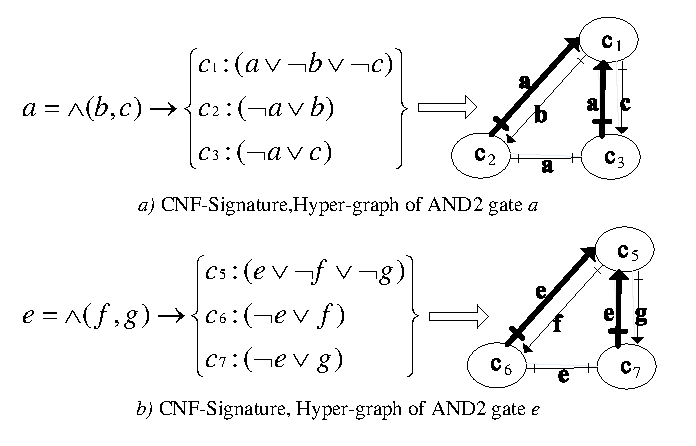
\includegraphics[width=7.2cm]{a6}
% \caption{CNF signature and Hyper-Graph of AND2 gate a and e}
% \label{fig_before}
% \end{figure}
% \begin{figure}[b]
% \centering
% 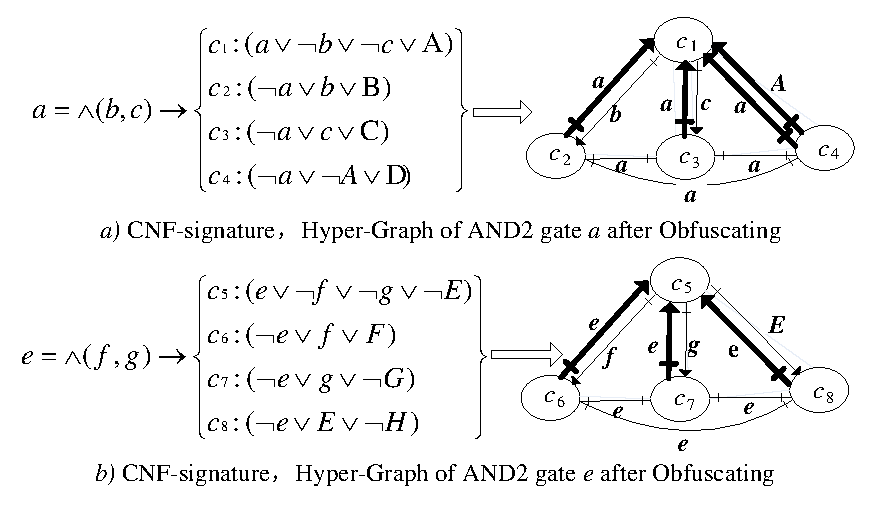
\includegraphics[width=7.2cm]{a7}
% \caption{CNF signature and Hyper-Graph of AND2 gate a and e after obfuscating}
% \label{fig_after}
% \end{figure}

\begin{figure}[b]
\centering
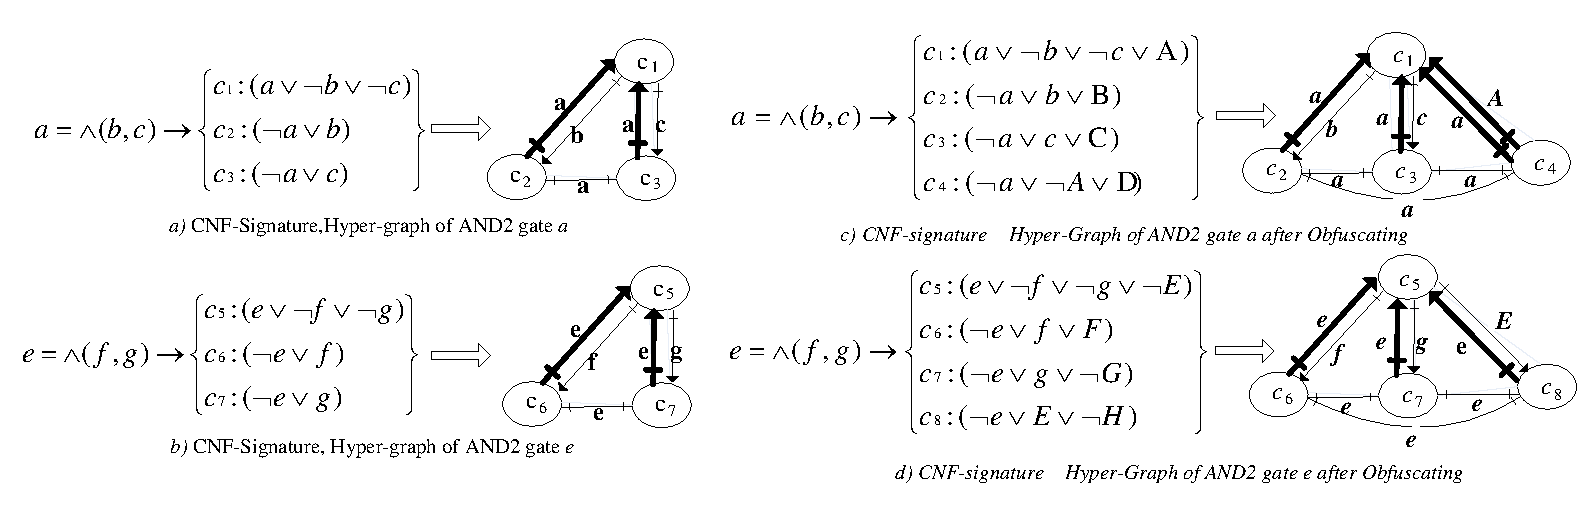
\includegraphics[width=13cm]{a6-1}
\caption{CNF signature and Hyper-Graph of $a$ and $e$ before and after obfuscating}
\label{fig_beforeafter}
\end{figure}

% Assume Husk result is $\{(F,F,F,F,T,F,T,T)\times(A,B,C,D,E,F,G,H)\}$.
Figure \ref{fig_beforeafter}a) and \ref{fig_beforeafter}b) shows the CNF signature and hyper-graph of two AND2 gate $a$ and $e$.
While their CNF signature and hypergraph after obfuscating are shown in Figure \ref{fig_beforeafter}c) and \ref{fig_beforeafter}d).
% By comparing Figure \ref{fig_beforeafter},
There are four types of changes:
\begin{enumerate}
 \item First, 
 the length of key clauses $c_1$ and $c_5$ are changed from 3 to 4, 
this defeats structure detection techniques \cite{t9} based on pattern matching key clause;
 \item Second, 
%  after obfuscating, 
 CNF signatures of $a$ and $e$ are changed.
%  thus their Hypergraph are not isomorphic anymore.
This defeats structure detection techniques\cite{t8} based on sub-graph isomorphic;
 \item Third, 
 there are new clauses added in formula, 
 such as $c_4$ and $c_8$, 
this change also defeats structure detection techniques\cite{t8} based on sub-graph matching;
 \item Furthermore, 
 by inserting proper literal in key clauses and generating new clause, 
 CNF signature of instance $e$ is changed from AND2 to AND3, 
as shown in Figure \ref{fig_beforeafter}b).
Husk variable $E$,
which becomes a input variable of gate AND3, 
is indistinguishable with $f$ and $g$,
which are original input variables of AND2.
this makes it impossible to distinguish AND2 and AND3. 
\end{enumerate}


The changes to bipartite graphs of $a$ and $e$ is similar. 

%Bipartite graphs of a and e, before and after obfuscating, are shown in fig.8 and fig.9.
%\begin{figure}
%\centering
%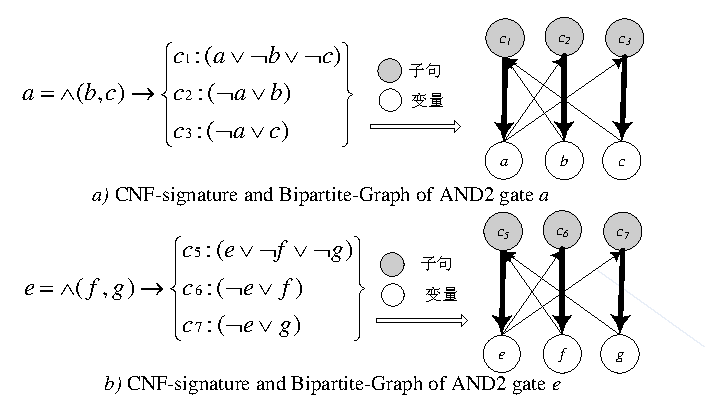
\includegraphics[width=7.2cm]{a8}
%\caption{Bipartite-Graphs of AND2 gate a and e}
%%\label{fig:example}
%\end{figure}

%Obfuscating brings changes to bipartite graphs of a and e, furthermore, bipartite graph of them are not isomorphic anymore.
%\begin{figure}
%\centering
%\includegraphics[width=7.2cm]{a9}
%\caption{Bipartite-Graphs of AND2 gate a and e after obfuscating}
%\label{fig:example}
%\end{figure}
%Analysis presented above only think about condition of inserting one variable into each clause, inserting more than one variable with different combination will bring more changes. 

% \subsubsection{Quantitative analysis} 
% 
% Pattern matching and sub-graph isomorphism are used to detect gate structures in CNF formula.
% Since key clause or CNF signature oriented pattern matching is dependent on key clause and CNF signature, changing them could prevent such attacks.
% Through searching isomorphic sub-graph, the gate structure with same CNF signature can be detected; thus even modifying the CNF signature of instances, 
% if instances of same type gate have the same new CNF signature, these instances can still be identified as the same type of gate through sub-graph isomorphism matching.
% After careful analysis, the orignal CNF signature may even be inferred. 
% 
% Therefore there are three level to measure changes to the CNF formula.
% The first level is to change key clause and characteristic clauses shown in 6a) and 7a);
% the second level is to change isomorphic relationship between CNF signature of instances, as shown in 7a) and 7b);
% the third level is to change CNF signature into distinguishable, 
% that is, even detecting the same CNF signature, 
% one is still unable to determine that two instances of the same CNF signature are corresponding to the same type of gate before obfuscating,
% as shown in Fig.7b) the instance of gateAND2 after obfuscating are distinguishable with instance of gate AND3 as shown in Fig5.
% 
% To measure the effectiveness, the following definitions are given.

% 
% \noindent \newline Definition 7: If using pattern matching technique can not detect instances of a type of gate in a CNF formulas, 
% CNF formula is called for such gate pattern matching attack safe, GPMA-safe.
% 
% \noindent \newline Definition 8: If In a CNF formula, some instances of the same type of gate are not isomorphic,
% the CNF formula is called for such gate partially isomorphic attack safe, GPIA-safe; If In a CNF formula,
% any two instances of the same type gate are not isomorphic, the CNF formula is called for such gate completely isomorphic attack safe, GCIA-safe.
% 
% \noindent \newline Definition 9: If in a CNF formula, same CNF signature may not be corresponds to same type of gate, the CNF formula is called for such gate structural safe, GS-safe.
% 
% \noindent \newline Definition 10: If in a CNF formula, any type of gate is GPMA-safe, the CNF formula is called pattern matching attack safe, PMA-safe.
% 
% \noindent \newline Definition 11: If in a CNF formula , there exists a type of gate which is GPIA-safe,
% the CNF formula is called PIA-safe; If in a CNF formula, every type of gate are GCIA-safe, the CNF formula is called CIA-safe.
% 
% \noindent \newline Definition 12: If in a CNF formula, any type of gate is GS-safe , the CNF formula is called S-safe. \noindent \newline {}  
% 
% Transforming a CNF formula into PMA-safe will increase the difficulty to recover circuit structure; 
% while transforming a CNF formula into PIA-safe can prevent complete circuit structure from detection; 
% futhermore  transforming a CNF formula into S-safe can prevent any part of circuit structure from detection.
% 
% \noindent \newline Definition 13: If there are n characteristic clauses in CNF signature of a certain type of gate, insert m literals into each clauses, 
% distinguished between positive or negative literal,the maximum number of new CNF signature for this gate can be derived is $T=(2^m)^n$ .
% When the number of instances is more than $T$, according to the drawer principle, 
% there must be 2 or more instances have the same new CNF signature, 
% thus through sub-graph isomorphic searching, one can detect gates which has same CNF signature.
% $T$ is Called isomorphic threshold.
% 
% For example, gate AND2 consists three characteristic clauses, when inserting one literal into each clauses, at most can derive $2^3=8$ new CNF signatures.
% If there are more than 8 gates AND2 in CNF formula, after obfuscating, there must be two or more gates which have same new CNF signature.
% In this case, the CNF formula can not be GCIA-safe for AND2, thus the CNF formula can not be CIA-safe.
% 
% % In OBFUSCATOR, two algorithms are implemented. one is randomly inserting a literal into each clause, then according the length of clause, inserting extra literals into short clauses.
% % The other is : first randomly inserting a literal into each clause; if clause is a key clause, then generate a clause with the inserted literal and output variable of key clause;
% % according the length of clause, insert extra literals into short clauses.
% 
% In OBFUSCATOR algorithms, first randomly inserting a literal into each clause; 
% if clause is a key clause, then generate a clause with the inserted literal and output variable of key clause;
% according the length of clause, insert extra literals into short clauses.
% %Assumed in CNF formula $S$, the number of a certain type of gate is $z$;
% %the number of characteristic clauses in CNF signature of the gate is $a$; 
% %the number of Husk literal used during obfuscating is x+y, 
% %including x positive literal and y negative literal;
% %the average number of literals inserted into clauses is n, 
% %according to both algorithms, n≥1. Thus isomorphic threshold T≥2a.
% %Under such conditions, the effectiveness of obfuscating is as following. 
% 
% %Table Effectiveness
% 
% % \noindent Algorithm 1:
% % 
% % Since algorithm inserts literal into to key clause so as to produce new clause, through original key clause based pattern matching, none gate can not be detected. CNF formual for gates is GPMA-safe. Thus the CNF formula is PMA-safe.
% % 
% % Condition1: the number of certain gates is more than its isomorphic threshold.
% % 
% % In worst case, literals inserted into each characteristic clause are all positive or negative. Since all new signatures are same, through sub-graph isomorphic detection, all gates of same type can be detected. Probability of the case occurs is shown in Table.
% % 
% % In best case, literals inserted into each characteristic clause are not all positive or negative. Since the number of certain gates is more than its isomorphic threshold, according to drawer principle, some gates must be transformed into same signature, the CNF formula is GPIA- safe for this gate. Thus the CNF formula is PIA-safe.
% % 
% % Condition2: the number of certain gates is not more than its isomorphic threshold.
% % 
% % In worst case, same as Condition1; In average case, some new signature may be transformed into same form,the CNF formula is GPIA- safe for this gate; Thus the CNF formula is PIA-safe. In best case, since number of gate is less than isomorphic threshold, all the signature may be transformed into different form, the CNF formula is GCIA- safe for this gate.
% % 
% % \noindent Algorithm 2:
% Since algorithm generates new clause according to key clause so as to produce new and legal signature, CNF formual for gates is GS-safe and GPMA-safe
% 
% \noindent Condition1: the number of certain gates is more than its isomorphic threshold:
% 
% In worst case, literals inserted into each key clause of the same type are all positive or negative, new signature of the gate are all same,thus through sub-graph isomorphic detection, all gates of this type can be detected.
% In average case and best case, literals inserted into each key clause are not all positive or negative. Since the number of certain gates is more than its isomorphic threshold, according to drawer principle, some new signature must be transformed into same form, the CNF formula is GPIA-safe for this gate. Thus the CNF formula is PIA-safe. 
% 
% 
% \noindent Condition2: the number of certain gates is not more than its isomorphic threshold.
% In worst case, same as Condition1; 
% 
% In average case, some new signature may be transformed into same form,the CNF formula is GPIA- safe for this gate; Thus the CNF formula is PIA-safe.
% 
% In best case, since number of gate is less than isomorphic threshold, all the signature may be transformed into different form, the CNF formula is GCIA- safe for this gate.

\subsection{Complexity of the algorithm analysis} 

% OBFUSCATOR1 consists only a layer of loop, thus the complexity of the algorithm is O (n); in OBFUSCATOR2 algorithm,procedureof marking key clause and output variable consists 2 layer of loops,complexity is O (n2), other part of algorithm consists only 1 layer of loop, the complexity of the algorithm is O (n2). The complexity of the algorithm is O MAPPER (n).
The main procedure of OBFUSCATOR algorithm consists only one layer of loop.
Although $\mathbf{mark}$ consists 4 layers of loop,
the runtimes of the 3 inner loops are bounded by length of clauses.
% so their complexity are still $O(n)$. 
% Other part of algorithm consists at most 1 layer of loop, 
So the complexity of the OBFUSCATOR algorithm is $O(n)$. 
The complexity of the MAPPER algorithm is obvious $O(n)$.

\section{Related works}\label{related}
% \subsection{Secure Computation Outsourcing}

% With the popularity of Cloud computing, secure outsourcing scientific computing become a hot research topic.
%in \cite{t5}\cite{t10}\cite{t12}\cite{t13}\cite{t14}\cite{t15}\cite{t17}\cite{t18}\cite{t21}.
% According to the methods used, it can be classified into encryption based method, disguising based method.
% and data partitioned based method.
% The difference between disguising and encryption lies in: 
% disguising does not change outsourcing algorithm, but only change the outsourced data. After disguising, 
% data can still hold a certain characteristics of the problem in order to obtain the final solution. 
% The method depends on the specific problems and specific methods of disguising, 
% the defect of the technique is lack of a uniform framework to protect data, 
% but the effect on performance is very small.With encryption based method, data and algorithm are isomorphic mapped into the encryption space. 
% This method can provide a unified framework to ensure data security, but the implementation overhead is very high.
% With data partitioned based method, data and computation are distributed so as to prevent entire data be acquired.    
% The related research will introduce in the following section.
\textbf{Secure Computation Outsourcing based on encryption:}
R. Gennaro et al.\cite{t16} presented the concept of verifiable computation scheme, 
% which is based on Yao’s Garbled-Circuit\cite{t38} and fully homomorphic encryption(FHE)\cite{t15},
which shows the secure computation outsourcing is viable in theory. 
But the extremely high complexity of FHE operation and the pessimistic circuit sizes make it impractical.
% that can hardly be handled in practice, 
% attempts to apply the scheme into real applications is still in progress.
Zvika et al.\cite{t12} constructed an obfuscated program for d-CNFs that preserves its functionality without revealing anything else. 
The construction is based on a generic multi-linear group model and graded encoding schemes, 
along with randomizing sub-assignments to enforce input consistency. 
But the scheme incurs large overhead caused by their fundamental primitives.
% such as computation cost by multi-linear map.

\textbf{Secure Computation Outsourcing based on disguising:}
% Instead of outsourcing general functions, in the security community, 
% Atallah et al. explore a list of customized solutions \cite{t19,t20,t21,t22} for securely outsourcing some specific computations. 
For linear algebra algorithms, 
Atallah et al. \cite{t19} multiplied data with random diagonal matrix before outsourcing. 
and recovered results by reversible matrix operations. 
But it had not discuss how to verify the result.
% The paper also discussed the extension problem domain and reduction, 
% in order to further disguise computation. 
% One problem with the approach is not discussed how to verify the correctness of the results returned.
Paper \cite{t20} discussed secure outsourcing of numerical and scientific computation,
by disguising with a set of problem dependent techniques.
% they explicitly allow private information leakage.
C.Wang\cite{t5} presented securely outsourcing linear programming(LP) in Cloud,
by explicitly decomposing LP computation into public LP solvers and private data, 
and provide a practical mechanism which fulfills input/output privacy, 
cheating resilience, and efficiency.
% \subsubsection{Partition based techniques}
% 
% Yuriy Brun\cite{t18} etc presented a approach named sTile to preserves the privacy of the computation data in 3-SAT. The sTile separates the computation into small subcomputations and distributes them in a way that makes it prohibitively hard to reconstruct the data. But for ease of the prototype implementation, sTile only implemented simple solving algorithms, without using efficient algorithms exists . network delay induced by sTile is still a problem to be solved.

\textbf{Verifiable computation delegation:}
Verifiable computation delegation is the technique to enable 
a computationally weak customer to verify the correctness of the delegated computation results
from a powerful but untrusted server without investing too much resources.
% has found great interests in theoretical computer science community.
% . propose a method of protecting high value rare events for general computation outsourcing in grid computing. 
To prevent participants from keeping the rare events, 
Du. et al. \cite{t17} injected a number of chaff items into the workloads so as to confuse dishonest participants.
% In distributed computing and targeting the specific computation delegation of one-way function inversion, 
Golle et al. \cite{t32} proposed to insert some pre-computed results (images of “ringers”) 
into the computation workload to defeat untrusted or lazy workers. 
Szada et al. \cite{t33} extended the ringer scheme and propose methods 
to deal with cheating detection.
% including optimization tasks and Monte Carlo simulations.
% Although these work mainly focus on results verification, the idea of addition of ringer, 
% garbled circuit or chaff instances into computation workload without investing too much resources illuminates us.

\section{Experiments}\label{exp}

Algorithms presented in this paper are all implemented in language $C$.
The experiments is conducted on a laptop with Intel Core(TM) i7-3667U CPU @ 2.00GHz, 8GB RAM. 
We unroll circuits in iscas89 benchmark for 30 times and transform them into CNF formulas,
and generate Husk formula with variables number $vn=675$ and clauses number $cn=2309$,
and then obfuscate the CNF formula.
Figure \ref{fig_exp} presents size of CNF formula after obfuscating with $vn$ and $cn$,
SAT Solver time(SAT Time) before and after obfuscating(CloudSAT Time),
obfuscating time(Obfuscating Time),
and result recovery time(Mapping time).


\begin{figure}
\centering
\includegraphics[width=10cm]{p1}
\caption{Relationship between Runtime and Size of CNF }
\label{fig_exp}
\end{figure}

Experiments show that, although the size of CNF formula($cn$ and $vn$) after obfuscating is increased,
SAT solver time does not follow a linear growth after obfuscating.
When the original CNF formula is much larger than the Husk formula,
SAT Solver time is likely to be the same between before and after obfuscating. 
% SAT solving time depends on the internal structure of CNF formula.
% On the other hand, 
At the same time,
obfuscating time and result recovering time increase linearly with the size of circuit 
(variables number and clauses number).

\section{Conclusion}\label{conclude}

% This paper is intended to meet the privacy-preserving needs of SAT solving in Cloud computing with disguising based techniques.
% A obfuscating algorithm changes the clauses set of CNF formula and literals set of clause so as to transform CNF signature in formula. 
% In the obfuscating process, with proper embedding rules,the algorithm remain the solution space of CNF formula unchanged, 
% namely: if the formula $S_1$  is unsatisfied, the formula $S$, which is gernerated by obfuscating $S_1$ , is unsatisfied either;
% If the formula $S_1$  is satisfied, the formula$S$can also be satisfied, 
% and furthermore, the solution of formula $S_1$  can be obtained by projecting solution of$S$ on set of variables of $S_1$  .
% 
% Due to obfuscating has transformed the characteristics clauses set of gate in formula,
% characteristics clauses based pattern matching can not restore the gate structure from CNF formula anymore.
% Since the obfuscating algorithm herein can not guaranteed all instances with the same type of CNF signature being transformed into different form, 
% the use of subgraph isomorphism methods may find a part of gate instances with same new signature,
% but it is still impossible to recover the full circuit structure. 
% Thorough security analysis and experiments demonstrate the effectiveness and practicality of the proposed mechanism.
This paper propose the first Cloud SAT solver algorithm 
that can prevent the confidential information in the CNF formula from being recovered by untrusted Cloud server.
Theoretical analysis and experimental result show that our algorithms can significantly improve security of the SAT solver 
with linear complexity while keeping its solution space unchanged.

% \section{Acknowledge} 
% 
% This work was supported by NSFC under grant.

% \section{REFERENCES} 

\begin{thebibliography}{4}


\bibitem{t1}	D.Putnam. A Computing Procedure for Quantification Theory. 
Journal of the ACM 7 (3): 201.
\bibitem{t2}	G. Hachtel, F. Somenzi.
Logic synthesis and verification algorithms. Springer 2006: I-XXIII, 1-564.
\bibitem{t3}	E. Clarke, O. Grumberg, S. Jha, Y. Lu, H. Veith.
Counterexample-Guided Abstraction Refinement. 
CAV'00, pp 154-169.
\bibitem{t4}	G. Tseitin. 
On the complexity of derivation in propositional calculus. Studies in Constr. Math. and Math. Logic, 1968.
\bibitem{t5}	C. Wang, K. Ren, J. Wang.
Secure and practical outsourcing of linear programming in Cloud computing. INFOCOM'11: 820-828.
\bibitem{t6}	C. Li.
Integrating equivalency reasoning into Davis-Putnam procedure. in AAAI'00, pp. 291-296.
\bibitem{t7}	R. Ostrowski. 
Recovering and exploiting structural knowledge from cnf formulas, CP'02, pp. 185-199.
\bibitem{t8}	J.Roy, I.Markov,V. Bertacco. 
Restoring Circuit Structure from SAT Instances IWLS'04, pp. 361-368.
\bibitem{t9}	Z. Fu, S. Malik. 
Extracting Logic Circuit Structure from Conjunctive Normal Form Descriptions. 
VLSI Design'07, pp 37-42.
\bibitem{t10}	MiniSat — SAT Algorithms and Applications Invited talk given by Niklas Sörensson at the CADE-20 workshop ESCAR. 
http://minisat.se/Papers.html
\bibitem{t11}	H. You.
Get Off of My Cloud: Exploring Information Leakage in Third-Party Compute Clouds, CCS'09
\bibitem{t12}	Z. Brakerski and G. Rothblum.
Black-Box Obfuscation for d-CNFs.
ITCS'14,pp. 235-250.
%\bibitem{t13}	Zvika Brakerski and Guy Rothblum. Obfuscating Conjunctions. CRYPTO 2013 Lecture Notes in Computer Science Volume 8043, 2013, pp 416-434. 
%\bibitem{t14}	Zvika Brakerski Cryptographic Methods for the Clouds Ph.D. Dissertation, Weizmann Institute of Science, 2011.
% \bibitem{t15}	C. Gentry, “Fully homomorphic encryption using ideal lattices,” in ACM STOC, Bethesda, MD, USA, 2009, pp. 169-178.
\bibitem{t16}	R. Gennaro, C. Gentry, B. Parno.
Non-interactive Verifiable Computing: Outsourcing Computation to Untrusted Workers.
CRYPTO'10, pp 465-482.
\bibitem{t17}	W. Du and M. Goodrich. 
Searching for High-Value Rare Events with Uncheatable Grid Computing.2004.
%\bibitem{t18}	Yuriy Brun and Nenad Medvidovic Keeping Data Private while Computing in the Cloud. IEEE CLOUD 2012: 285-294
\bibitem{t19}	M. Atallah, K. Pantazopoulos, J. Rice, E. Spafford.
Secure outsourcing of scientific computations. 
Advances in Computers 54: 215-272 (2001)
\bibitem{t20}	M. Atallah, J. Li.
Secure outsourcing of sequence comparisons.
Int. J. Inf. Sec. 4(4): 277-287 (2005).
% \bibitem{t21}	David Benjamin, Mikhail J. Atallah: Private and Cheating-Free Outsourcing of Algebraic Computations. PST 2008: 240-245
% \bibitem{t22}	Mikhail J. Atallah, Keith B. Frikken: Securely outsourcing linear algebra computations. ASIACCS 2010: 48-59
%\bibitem{t23}	Dimitris Achlioptas、Carla Gomes、Henry Kautz、Bart Selman . Generating Satisfiable Problem Instances. 12th National Conference on Artificial Intelligence (AAAI-2000) 2000, 256-301
% \bibitem{t24}	Tuomo. Factoring benchmark for SAT-solover
%\bibitem{t25}	Harri H,Matti J,Petteri K,Ilkka N. Hard Satisfiable Clause Sets for Benchmarking Equivalence Reasoning Techniques. Journal on Satisfiability, Boolean Modeling and Computation 2 (2006) 27-46%
%\bibitem{t26}	Matti J ̈rvisalo  Equivalence checking hardware multiplier designs SAT Competition 2007 - benchmark description
%\bibitem{t27}	Adi Shamir. How to share a secret. Communications of the ACM, Volume 22 Issue 11, Nov. 1979.
%\bibitem{t28}	Ronald L. Rivest, Adi Shamir, Leonard M. Adleman: A Method for Obtaining Digital Signatures and Public-Key Cryptosystems. Commun. ACM 21(2): 120-126 (1978)
%\bibitem{t29}	Taher El Gamal: A public key cryptosystem and a signature scheme based on discrete logarithms. IEEE Transactions on Information Theory 31(4): 469-472(1985)
%\bibitem{t30}	Shafi Goldwasser, Silvio Micali: Probabilistic Encryption and How to Play Mental Poker Keeping Secret All Partial Information STOC 1982: 365-377
% \bibitem{t31}	P. Paillier.
% Public-Key Cryptosystems Based on Composite Degree Residuosity Classes. 
% EUROCRYPT'99, pp. 223-238.
\bibitem{t32}	P. Golle and I. Mironov.
Uncheatable distributed computations.
CT-RSA'01, pp. 425–440.
\bibitem{t33}	D. Szajda, B. G. Lawson, and J. Owen.
Hardening functions for large scale distributed computations.
ISSP'03, pp. 216-224.
%\bibitem{t34}	Marina Blanton, Yihua Zhang, Keith B. Frikken: Secure and Verifiable Outsourcing of Large-Scale Biometric Computations. SocialCom/PASSAT 2011: 1185-1191
\bibitem{t35}	Paralleling OpenSMT Towards Cloud Computing http://www.inf.usi.ch/urop-Tsitovich-2-127208.pdf‎
%\bibitem{t36}	Jan Krajícek: Interpolation Theorems, Lower Bounds for Proof Systems, and Independence Results for Bounded Arithmetic. J. Symb. Log. 62(2): 457-486 (1997)
\bibitem{t37}	Formal in the Cloud OneSpin’s New Spin on Cloud Computing.http://www. eejournal.com/archives/articles/20130627-onespin/?printView=true
% \bibitem{t38}  A. C.-C. Yao, “Protocols for secure computations (extended abstract),” in Proc. of FOCS, 1982, pp. 160-164.

\end{thebibliography}
\end{document}
